\documentclass[]{article}

% Imported Packages
%------------------------------------------------------------------------------
\usepackage{amssymb}
\usepackage{amstext}
\usepackage{amsthm}
\usepackage{amsmath}
\usepackage{color}
\usepackage{enumerate}
\usepackage{fancyhdr}
\usepackage[margin=1in]{geometry}
\usepackage{graphicx}
\usepackage{extarrows}
\usepackage{setspace}

% \renewcommand*\familydefault{\sfdefault}
% \usepackage{cmbright}
% \usepackage{helvet}
%------------------------------------------------------------------------------

% Header and Footer
%------------------------------------------------------------------------------
\pagestyle{plain}
\renewcommand\headrulewidth{0.4pt}
\renewcommand\footrulewidth{0.4pt}
%------------------------------------------------------------------------------

% Title Details
%------------------------------------------------------------------------------
\title{
  Erudite\\
  \large \emph{An educational content management system}  \\
    \color{red} NOT FOR REMARKING
}

\author{
  SE 3A04: Software Design II -- Large System Design\\
  \\
  \begin{tabular}{ l l }
    Kelvin Lin*   & STUDENT-NUM \\
    Danish Khan   & STUDENT-NUM \\
    Puru Jetly    & STUDENT-NUM \\
    Terrance Yip  & STUDENT-NUM \\
    Varun Hooda   & STUDENT-NUM \\
  \end{tabular}
}

\date{}
%------------------------------------------------------------------------------

% Document
%------------------------------------------------------------------------------
\begin{document}

\maketitle
\newpage

\tableofcontents
\newpage


\section{Introduction}
\label{sec:introduction}
This section outlines the purpose and scope of the Erudite project; along with
definitions, acronyms and abbreviations used within this document; and finally
an overview of the contents and organization of this software requirements
document.


\subsection{Purpose}
\label{sub:purpose}
This document's purpose is to outline the engineering and business decisions
made in the design portion of the Erudite project. This document will be
used to maintain a record of project's scope, constraints, assumptions,
dependencies, functional requirements, non-functional requirements and any
other design decision made over the life of this project.

The target audience for this document are the stakeholders (Dr. Ridha Khedri,
Andrew Le Clair and Michael Liut), and any current or future architects,
designers and developers of this project.


\subsection{Scope}
\label{sub:scope}
This project will produce the following software products:
\begin{itemize}
  \item \underline{Android} client application
  \item Back-end web server
  \item Back-end database server
\end{itemize}

\noindent The aforementioned products preform the following:
\begin{itemize}
  \item Provide users with a graphical client-side application for creating,
    modifying and viewing server hosted content.
  \item Provide a means of retrieving and sending data between the front-end
    client and back-end web server.
  \item Provide a means of persistent storage and retrieval of content.
\end{itemize}

\noindent The aforementioned products do not preform the following:
\begin{itemize}
  \item Generate content.
\end{itemize}

\noindent These software products will combine to provide a content management
system for teachers and students in an educational environment. Benefits include
quick
access to educational content, efficient management of content, portability,
ease of access to content, and ease of assessing student-submitted material
(i.e. quizzes, assignments, etc). The goals of this project include providing
students and teachers with a familiar
interface to access and add content, all the while reducing any additional
overhead of maintaining a system, and providing easy accessibility to all
users.



\subsection{Definitions, Acronyms, and Abbreviations}
\label{sub:definitions_acronyms_and_abbreviations}
\begin{description}
  \item [Access Rights] See Permissions.

  \item [Android] An Unix-based operating system developed by Google Inc. for
    electronic devices including but not limited to touch-enabled
    \underline{smartphones},
    tablets, and other portable computing devices.

  \item [Classroom Operations] The set of typical actions performed in a
    classroom.

  \item [CMS] Content Management System. A system capable of hosting, managing
	and delivering digital content to a user.

  \item [LMS] Learning Management System. A specific instance of a Content
    Management System with an emphasis on educational or learning materials and
    institutions.

  \item [Mechanism of Assessment] Assignments, quizzes, and other ways of
    assessing and evaluating a students knowledge.

  \item [Metric of Success] Means of measuring a student's knowledge (grades,
    points, stars, percentage, etc.).

  \item [Permissions] The set of allowed actions a user is able to perform.

  \item [Smartphone] An embedded electronic device capable of serving as a
    general purpose, internet-enabled computer in addition to providing mobile
    telephone functionality such as phone calls and text messaging.

  \item [Teaching Methods] Ways of teaching including but not limited to
    assignments, examinations and tests.

  \item [User Role] Categorization of the user into a set of possible
    institutional roles (administration, teacher, student).

  \item [Course] A collection of \underline{course content}, \underline{student
    content} and student grades.

  \item [Course Content] Content that is one of three types: \underline{course
    material}, \underline{course assignment} or \underline{course assessment}.

  \item [Student Content] Content that is one of two types: \underline{student
    assignment} or \underline{student assessment}.

  \item [Course Material] All course content to which students cannot submit
    content in reply. This type of course content consists of but is not
    limited to .pdf, .ppt or .txt file types. This content may be set
    \underline{visible} or invisible for a specified duration of time.
    Non-evaluational content and course material are synonymous.

  \item [Course Assignment] Course content to which students may submit content
    in reply. Content submitted in reply is called a submitted student
    assignment.  Course assignments are of but is not limited to .pdf, .ppt or
    .txt file types. This content may be set visible or invisible for a
    specified duration of time (including infinitely long). Manual-evaluational
    content and course assignment are synonymous.

  \item [Course Assessment] Course content which students may submit. A
    submitted Course Assessment is called a student assessment. Course
    assessments may be in the form of, but not limited to, .pdf or .txt.
    Automated-evaluational content and course assessment are synonymous.

  \item [Student Assignment] Content that the student submits in reply to a
    course assignment type content.

  \item [Student Assessment] Content in which a download option is not
    provided.  This type of content typically consists of a questionnaire in
    which every question has at least two possibly correct choices. Students
    answer the questionnaire by picking at least on of the available options or
    inputting a textual response and submit before a specified time or submit
    automatically after a specified amount of time. The results are evaluated
    by the system and a student performance is recorded.

  \item [Visible] An attribute that can be assigned to a \underline{course},
    course content or student content. If assigned to a course, that course
    becomes open to all students for enrolment. If assigned to course content
    or student content, that content is then made available to be viewed to all
    students enrolled within that course.

\end{description}

\subsection{References}
\label{sub:references}
This section is void.


\subsection{Overview}
\label{sub:overview}
The rest of this documents contains detailed descriptions of this projects
design decisions: assumptions, functionality, functional requirements and
non-functional requirements.

The other sections are organized into logical subsections. Specifically, Section
2 outlines the overall product description with various subsections. Then the
following sections list the requirements. The functional requirements are
organized by business events and viewpoints. Non-functional requirements are
organized into various subcategories.


% End Section


\section{Overall Description}
\label{sec:overall_description}
% Begin Section

This section of the document describes the general factors that affect the
product and its requirements, providing context for the requirements in the
following sections.

\subsection{Product Perspective}
\label{sub:product_perspective}
% Begin SubSection
Erudite is a distributed learning management system designed to facilitate
teachers and students with everyday \underline{classroom operations}. Erudite is
a distributed, self-contained system with several components running on
different end-user devices. Erudite is akin to other learning management
systems, such as McMaster's Avenue2Learn; however, Erudite will focus on
providing a Learning Management System for early learners and educators with
low levels of technical expertise.

Figure 1 shows an overview of the major system components of the system as well
as their external interfaces.

\begin{figure}[h]
  \centering
  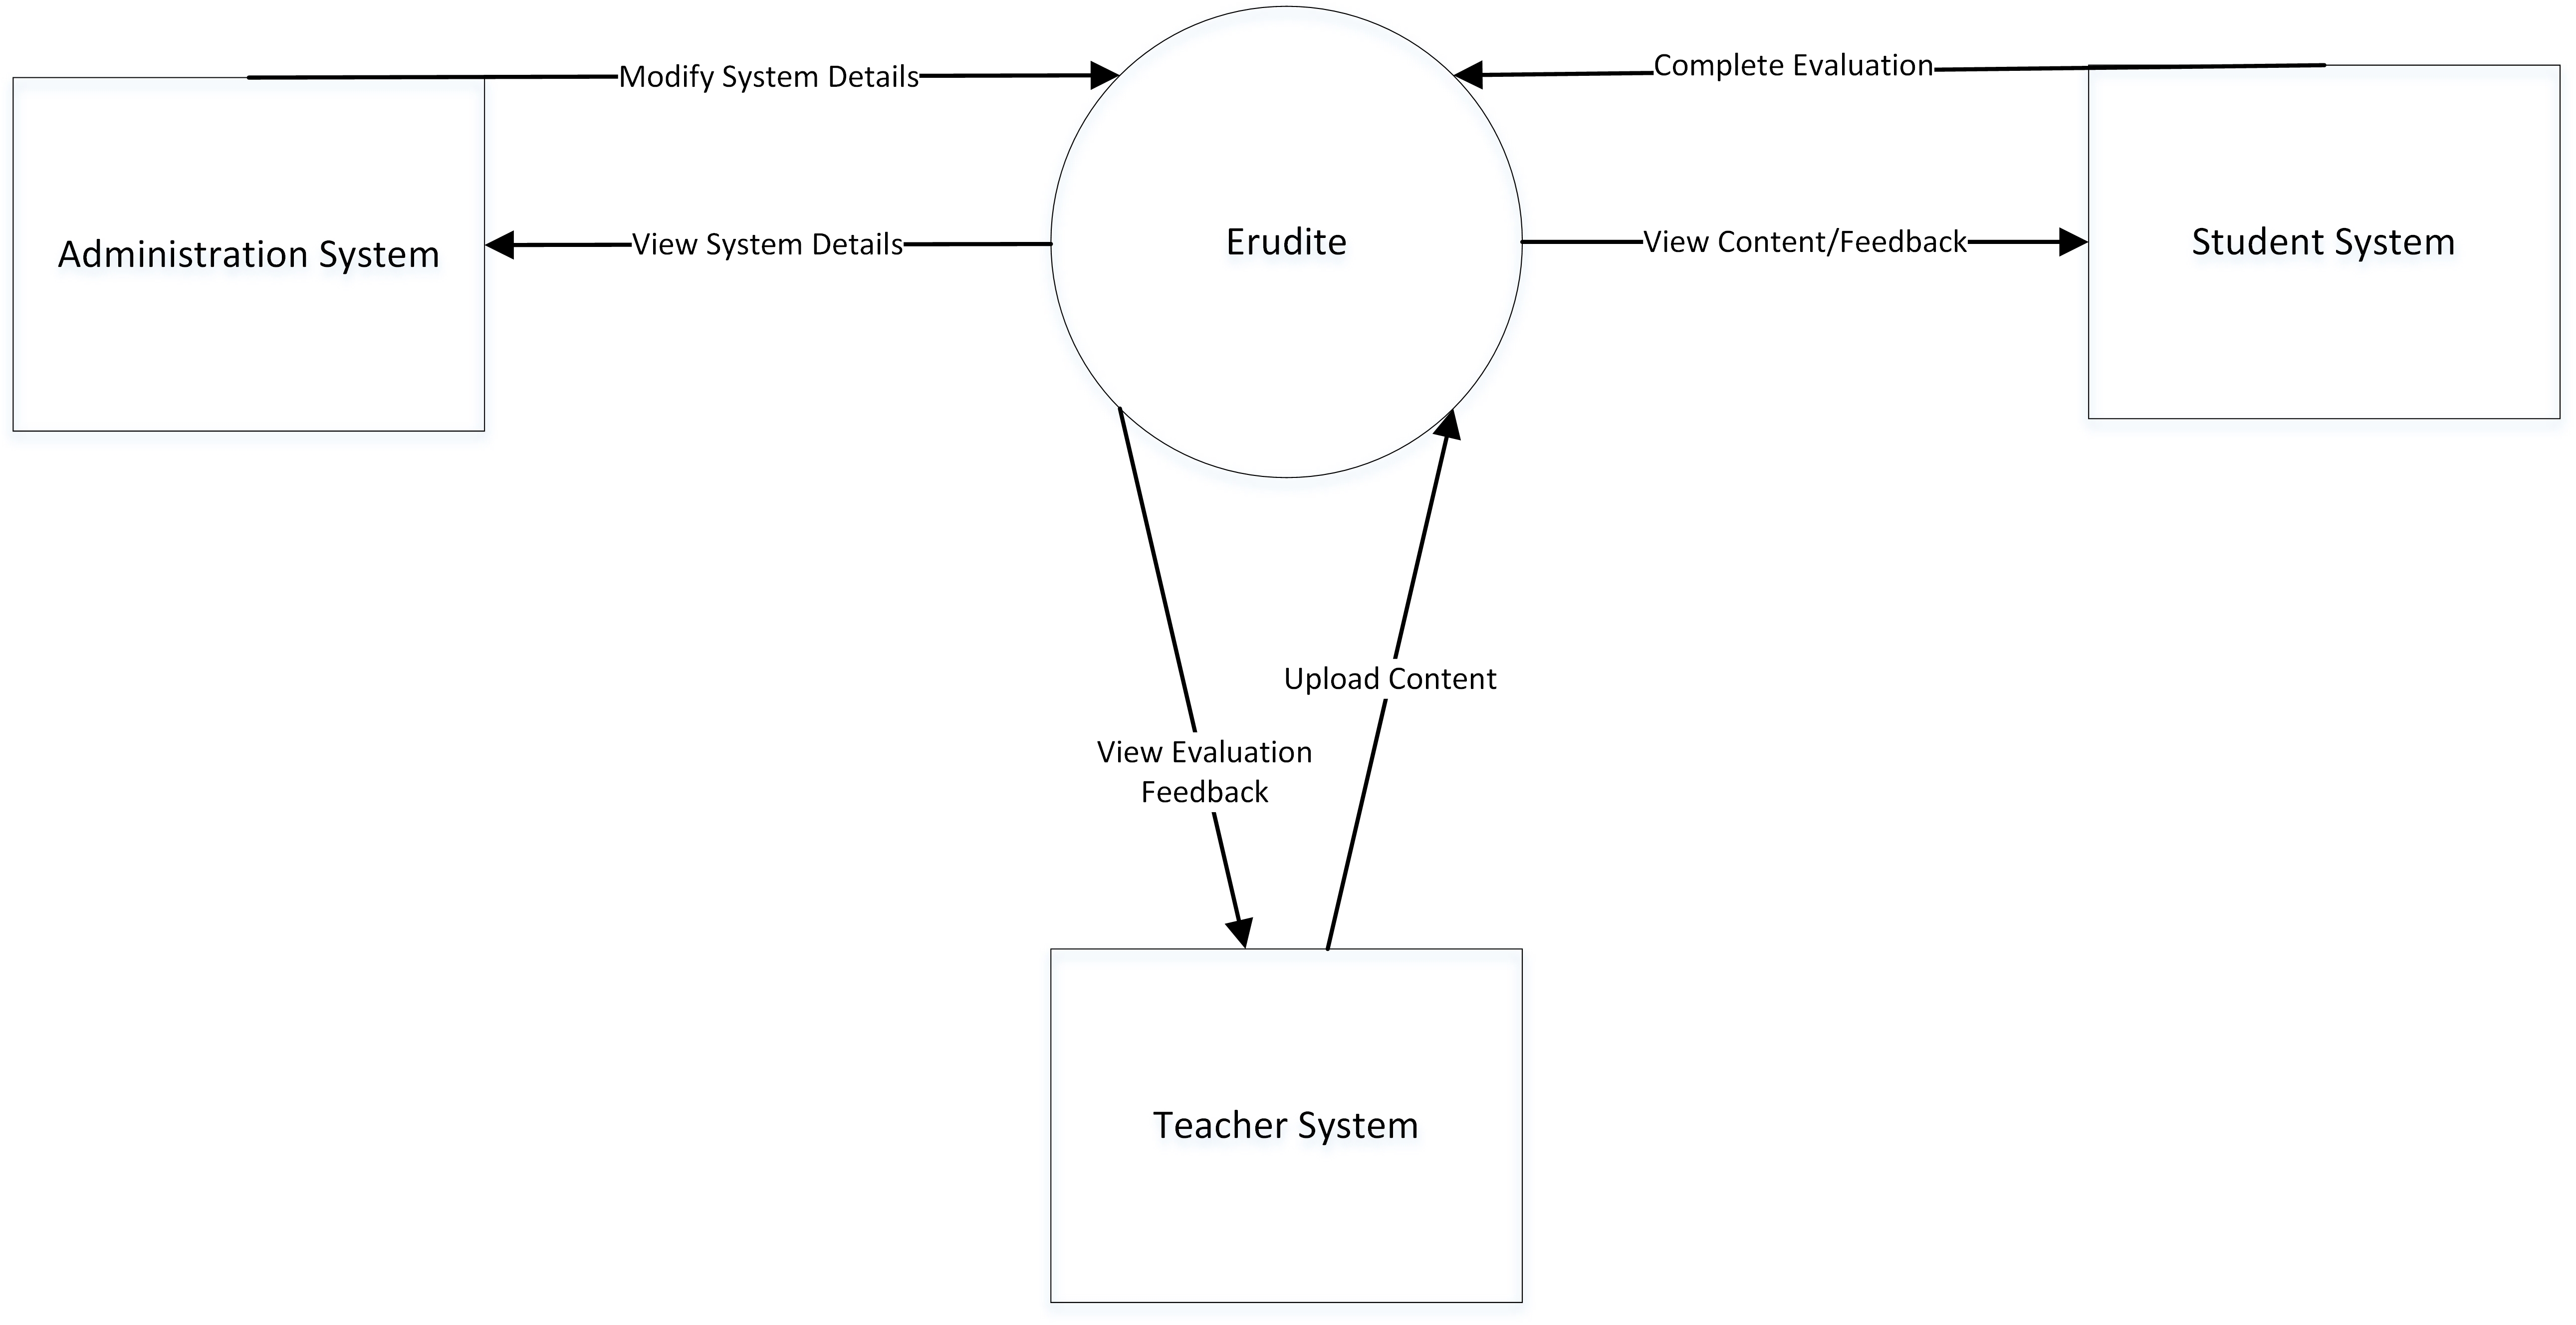
\includegraphics[scale=0.7]{A1_Assets/2-1_Product_Perspective_Diagram_v2.jpg}
  \caption{Major components of the system and their external interfaces.}
\end{figure}


% End SubSection

\subsection{Product Functions}
\label{sub:product_functions}
% Begin SubSection
Erudite is designed to facilitate students, teachers, and administration
with common classroom operations.

As a \underline{LMS}, Erudite will allow teachers to upload a variety of
documents for
the purpose of education. Teachers are then able to set the duration that the
documents are available, as well as the \underline{access rights} users
have over the document.

Moreover, Erudite will allow teachers to create virtual mechanisms of
assessment including but not limited to quizzes and electronic assignment
submission boxes. With virtual quizzes, teachers will be able to create their
own questions and solutions.

Teachers will also be able to configure settings related to these mechanisms of
assessment including but not limited to the availability of the mechanism,
functionalities available while users are participating in the mechanism of
assessment, and the assessment scheme associated with the mechanism.

The LMS will also allow teachers to enter success metrics for each student. If
instructed to do so, the LMS will also be able to automatically assess students
based on primitive assessment schemes provided by the teacher.

Erudite will allow teachers to view statistics associated with each
\underline{mechanism of assessment}. It will create visualizations of data
generated from the results of the assessment scheme and display them to the
teacher. Statistics to be displayed to the teacher include but is not limited
to the statistical mean, the statistical mode, the variance, the standard
deviation, the point biserial, and the discrimination index. \emph{\textbf{ An
innovative feature of Erudite is that it will also keep track of the number of
students who have yet to submit relevant work to each mechanism of assessment
so that teachers may be able to contact the class to remind them of the due
date, or extend the due date.}}

On the other hand, Erudite will allow students to view documents uploaded by
the teacher. The students will be able to save a copy of the document if it is
allowed by the teacher.

Moreover, Erudite will allow students to complete virtual mechanisms of
assessments created by their teacher. The LMS will allow students to submit the
appropriate information in order to successfully complete the mechanism of
assessment. The LMS will show the student a \underline{metric of success} when
authorized by the teacher.

\emph{ \textbf{
  Erudite will allow students and teachers to customize their own user
  interface such that information each user considers relevant will be
  displayed in a convenient location. Users will also have the option of adding
  other data including but not limited to weather information, traffic
  information, and the current time.
} }

Finally, Erudite will allow administration to add or remove students from
certain domains. The LMS will allow administration to modify the
\underline{user roles} and to control what \underline{permissions} each role
has over the system.
% End SubSection

\subsection{User Characteristics}
\label{sub:user_characteristics}
% Begin SubSection
Erudite is intended for 3 primary groups of users: teachers, students, and
administration.

Teachers are assumed to be adult users with the functional capacity of an
average person who is between the ages of 16 and 80. Teachers are assumed to be
fluent in written English, and have at least a basic understanding of
mathematics and statistics if they would be interested using the various
mathematical/statical data visualization features provided by the system.
Moreover, teachers are assumed to have a strong understanding of
\underline{teaching methods}; however, teachers are not assumed to be
well-versed in technology. Teachers should know how to use an Android platform
- including typing and selecting elements on the screen - however, they are not
expected to know how to know advanced features of the Android platform.

Students are assumed to be child users of ages 6 to 13, who are enrolled in a
Canadian, American, or culturally equivalent elementary school. Students are
assumed to understand basic written English at the Ontario Senior
Kindergarten/Grade 1 level. Students are expected to have vision and are able
to use the basic functions of the Android platform, albeit at a lower level
than teachers and administrations. At a minimum, students are assumed to know
how to select elements on the screen. No other prior knowledge is assumed of
the student.

The administration is assumed to be adult users with the functional capacity of
an average person who is between the ages of 16 to 80. The administration is
assumed to be fluent in written English, and have a good understanding of
mathematics and statistics. The administration is also assumed to have basic
computer knowledge, including basic troubleshooting, IT, and data entry skills.
The administration is assumed to have an intermediate understanding of common
Android platform usage, and are able to preform more advanced tasks such as
set-up, installation, and troubleshooting on such platforms.
% End SubSection

\subsection{Constraints}
\label{sub:constraints}
% Begin SubSection
The application must run on the native Android platform, as per the project
specifications provided.
% End SubSection

\subsection{Assumptions and Dependencies}
\label{sub:assumptions_and_dependencies}
% Begin SubSection
It is assumed that the school using the system will have the necessary
infrastructure to support the system. The school will provide the required
hardware in order to reasonably ensure the security of the data, and to handle
the data capacity requirement.

Moreover, it is assumed that each user will have access to an Android platform
that is internet enabled.
% End SubSection

\subsection{Apportioning of Requirements}
\label{sub:apportioning_of_requirements}
% Begin SubSection
\begin{enumerate}[{BE}1.]
	\item A teacher wants to create a course.
	\begin{enumerate}[{VP1}.1]
		\item Student Viewpoint
			\begin{enumerate}
				\item Students shall be able to enrol in an existing course owned by the
teacher provided the course is set visible.
			\end{enumerate}
		\item Teacher Viewpoint
			\begin{enumerate}
			    \item The teacher shall own the created course.
				\item A teacher shall be able to choose to unenroll a student from a course
that the teacher owns.
				\item A teacher shall not be enrolled in a course.
			\end{enumerate}
		\item Parent Viewpoint
			\begin{enumerate}
				\item Parents shall be able to view the course's progress or student
performance through their child's account.
			\end{enumerate}
		\item School Administration Viewpoint
			\begin{enumerate}
				\item The school administration shall be allowed to choose to whether to
allow students and teachers
to create their own accounts, or create accounts for all students and teachers.
			\end{enumerate}
		\item Information Technology Team Viewpoint
			\begin{enumerate}
				\item None
			\end{enumerate}
		\item Government \& School Board Viewpoint
			\begin{enumerate}
				\item All courses, course content, student content and any teacher student
communication held on the on the system shall be made visible to the school
board.
			\end{enumerate}
	\end{enumerate}

	\item A teacher wants to add content to a course they own.
	\begin{enumerate}[{VP1}.1]
		\item Student Viewpoint
			\begin{enumerate}
        \item A student enrolled in a course shall be able to view any content 
within the course when the content is set visible by the owner of that course.
        \item The system shall provide interface elements that allow the student 
to view any content set visible by the course owner.
        \item A student shall be able to submit an \underline{assignment}; a 
piece of content uploaded in response to a manual-evaluational content when the 
manual-evaluational content is set visible by the owner of that course and file 
submission is enabled.
        \item The system shall provide interface elements that allow the student 
to submit an assignment in response to manual-evaltional content.
        \item A student shall be able to submit an automated-evaluational 
content when it is set visible by the owner of that course.
        \item The system shall provide interface elements that allow the student 
to open and submit automated-evaluational content that is set visible by the 
owner of the course.
			\end{enumerate}
		\item Teacher Viewpoint
			\begin{enumerate}
				\item Teachers shall be allowed to set permissions that students have over 
each file.
        \item The system shall provide interface elements that allow the teacher 
to set permissions that students have over each file.
				\item The teacher shall specify a time period for which file submission is 
accepted by the manual-evaluational piece of content for manual-evaluational 
content.
        \item The system shall provide interface elements that allow the teacher 
to speicify the time period for which file submission is accepted by 
manual-evaluational content.
			\end{enumerate}
		\item Parent Viewpoint
			\begin{enumerate}
				\item None
			\end{enumerate}
		\item School Administration Viewpoint
			\begin{enumerate}
				\item None
			\end{enumerate}
		\item Information Technology Team Viewpoint
			\begin{enumerate}
				\item None
			\end{enumerate}
		\item Government \& School Board Viewpoint
			\begin{enumerate}
				\item None
			\end{enumerate}
	\end{enumerate}

	\item A teacher wants to add automated-evaluational content.
	\begin{enumerate}[{VP2}.1]

		\item Student Viewpoint
			\begin{enumerate}
        \item Students shall be able to view the automated-evaluational content
          only if the teacher sets the visibility of the content to be viewable
          by students.

        \item Students shall be able to open automated-evaluational content for
          a predefined period of time specified by the course owner when the
          content is made visible.

        \item Automated-evaluational content that has been opened and viewed by
          a student shall be submitted manually by the student or automatically
          before or at the end of predefined time (as specified by the teacher)
          respectively.
			\end{enumerate}

		\item Teacher Viewpoint
			\begin{enumerate}
        \item The teacher shall specify the visibility of the
          automated-evaluational content or it will default to "not visible to
          students".
			\end{enumerate}

		\item Parent Viewpoint
			\begin{enumerate}
				\item None
			\end{enumerate}

		\item School Administration Viewpoint
			\begin{enumerate}
				\item None
			\end{enumerate}

		\item Information Technology Team Viewpoint
			\begin{enumerate}
				\item None
			\end{enumerate}

		\item Government \& School Board Viewpoint
			\begin{enumerate}
				\item None
			\end{enumerate}

	\end{enumerate}

  \item The owner of a course specifies a time period in which non-evaluational
    content, manual-evaluational content, automated-evaluational content or a
    course is set visible for all enrolled students.
	\begin{enumerate}[{VP2}.1]

		\item Student Viewpoint
			\begin{enumerate}
        \item Students shall be unenrolled from a course that is set to not
          visible.

        \item Students shall not be able to view a course or
          \textbf{course content} which is not made visible to them.
			\end{enumerate}

		\item Teacher Viewpoint
			\begin{enumerate}
        \item The teacher shall be able to permanently remove \textbf{course
          content} from a course owned by them.
			\end{enumerate}

		\item Parent Viewpoint
			\begin{enumerate}
				\item None
			\end{enumerate}

		\item School Administration Viewpoint
			\begin{enumerate}
				\item None
			\end{enumerate}

		\item Information Technology Team Viewpoint
			\begin{enumerate}
				\item None
			\end{enumerate}

		\item Government \& School Board Viewpoint
			\begin{enumerate}
				\item None
			\end{enumerate}
	\end{enumerate}

  \item A student attempts to enroll in a course.
	\begin{enumerate}[{VP2}.1]
		\item Student Viewpoint
			\begin{enumerate}
        \item A student shall not be able to enroll in a course that is not
          visible to them.
        \item A student shall be able view all courses in which they are
          enrolled.
        \item A student shall not be able to self withdraw from a course in
          which he or she is enrolled.
        \item A student that is dismissed from a course shall no longer be
          enrolled in that course.
        \item A dismissed student shall not self enroll in a course from which
          he or she was dismissed.
        \item A student whom is not enrolled in a course shall have no access
          to \textbf{course content} found within that course.
			\end{enumerate}
		\item Teacher Viewpoint
			\begin{enumerate}
        \item A teacher shall be able to dismiss an enrolled student from a
          course owned by that teacher.
			\end{enumerate}
		\item Parent Viewpoint
			\begin{enumerate}
				\item None
			\end{enumerate}
		\item School Administration Viewpoint
			\begin{enumerate}
        \item The school administration shall be able to dismiss an enrolled
          student from a course.
			\end{enumerate}
		\item Information Technology Team Viewpoint
			\begin{enumerate}
				\item None
			\end{enumerate}
		\item Government \& School Board Viewpoint
			\begin{enumerate}
				\item None
			\end{enumerate}
	\end{enumerate}


	\item The school administration wants to add a Teacher or a Student account.
	\begin{enumerate}[{VP1}.1]
		\item Student Viewpoint
			\begin{enumerate}
				\item The student shall receive a Student ID and password to access their
personal if a new student account.
				\item The system shall allow the student to access their personal account 
when given the correct student id and password.
				\item The student shall choose a new password upon first signing into the
system.
				\item The system shall prompt new users to change their password.
			\end{enumerate}
		\item Teacher Viewpoint
			\begin{enumerate}
				\item The teacher shall receive a Teacher ID and password to access their
personal teacher account.
				\item The system shall allow a teacher to access their personal account 
given the correct login credentials.
				\item The teacher shall choose a new password upon first signing into the
system.
				\item The system shall prompt new users to change their password.
			\end{enumerate}
		\item Parent Viewpoint
			\begin{enumerate}
				\item None
			\end{enumerate}
		\item School Administration Viewpoint
			\begin{enumerate}
				\item The School Administration shall be able to create a set of usernames
and passwords from an external file.
				\item The system shall store a set of usernames and passwords.
			\end{enumerate}
		\item Information Technology Team Viewpoint
			\begin{enumerate}
				\item None
			\end{enumerate}
		\item Government \& School Board Viewpoint
			\begin{enumerate}
				\item The school administration shall monitor communication.
				\item The system shall provide functionality for the school administration 
to monitor communication
				\item All enquiries shall be
forwarded to the school administration.
				\item The system shall forward all enquiries to the school administration.
				\item The school
administration shall be given access and privileges to hide, remove or track the
origin of a piece of content or course when any content malign against board
policies is uploaded to the system.
				\item The system shall have privileges that are provided to the school 
administration to remove and track origins of a piece of content or course.
			\end{enumerate}
	\end{enumerate}

	\item The school administration wants to delete a course.
	\begin{enumerate}[{VP1}.1]
		\item Student Viewpoint
			\begin{enumerate}
				\item All students shall be unenrolled from the course.
				\item The system shall allow student to be unenrolled from courses.
			\end{enumerate}
		\item Teacher Viewpoint
			\begin{enumerate}
				\item A teacher shall not own a deleted course.
				\item The system shall check that no teachers have a deleted course.
				\item{All content shall be deleted from the system.}
				\item The system shall delete all the content from a deleted course.
			\end{enumerate}
		\item Parent Viewpoint
			\begin{enumerate}
				\item None
			\end{enumerate}
		\item School Administration Viewpoint
			\begin{enumerate}
				\item The school administration account shall be given a warning after a
course
deletion request is made.
				\item The system shall alert the school administration when deletion request 
is made.
\item The course shall deleted only if a course deletion
request is made a second time following the warning.
\item The system shall only allow the course to be deleted after another 
deletion request is made after the warning.
			\end{enumerate}
		\item Information Technology Team Viewpoint
			\begin{enumerate}
				\item None
			\end{enumerate}
		\item Government \& School Board Viewpoint
			\begin{enumerate}
				\item None
			\end{enumerate}
	\end{enumerate}
\end{enumerate}
% End SubSection

% End Section

\section{Functional Requirements}
\label{sec:functional_requirements}

Please refer to \textbf{Section 1.3 Definitions, Acronyms, and Abbreviations}
for a definitions of \textbf{key} terms used herein.

% TEACHER BUSINESS EVENTS (5)

\begin{enumerate}[{BE}1.]	
	\item A teacher views a submitted \underline{student assignment}.
	\begin{enumerate}[{VP2}.1]
		\item Student Viewpoint
			\begin{enumerate}
				\item A student shall be able to submit a \underline{student assignment} multiple times in response to a manual-evaluational content posted by the course owner when the manual-evaluational content is set visible by the course owner and file submission is enabled for that manual-evaluational content.
        \item The system shall allow the student to submit a \underline{student assignment} multiple times in response to a visible manual-evaluational content and for which file submission is enabled.
			\end{enumerate}
		\item Teacher Viewpoint
			\begin{enumerate}
				\item A teacher shall be able to change an assigned weight or grade to a \underline{student assignment}.
        \item The system shall provide interface elements that allow the teacher to change an assigned grade to a \underline{student assignment}.
				\item The teacher shall define the numerical value of each letter grade. The values of each letter grade can be redefined by the teacher.
        \item The system shall provide interface elements that allow the teacher to define the numerical value of each letter grade within a course.
			\end{enumerate}
		\item Parent Viewpoint
			\begin{enumerate}
				\item None
			\end{enumerate}
		\item School Administration Viewpoint
			\begin{enumerate}
				\item None
			\end{enumerate}
		\item Information Technology Team Viewpoint
			\begin{enumerate}
				\item None
			\end{enumerate}
		\item Government \& School Board Viewpoint
			\begin{enumerate}
				\item None
			\end{enumerate}
	\end{enumerate}


% STUDENT BUSINESS EVENTS (4)

  \item A student wants to check their grades.
	\begin{enumerate}[{VP2}.1]
		\item Student Viewpoint
			\begin{enumerate}
        \item The system shall calculates and display an overall grade for a
          given course and an overall grade point average for all courses the
          student is enrolled in.
        \item If no grades are assigned, the system shall not display an
          overall grade for a given course.
        \item If the student is not enrolled in any courses or no grades are
          assigned for every course the student is enrolled in, an overall
          grade point average for all courses shall not be displayed.
			\end{enumerate}
		\item Teacher Viewpoint
			\begin{enumerate}
				\item None
			\end{enumerate}
		\item Parent Viewpoint
			\begin{enumerate}
				\item None
			\end{enumerate}
		\item School Administration Viewpoint
			\begin{enumerate}
				\item None
			\end{enumerate}
		\item Information Technology Team Viewpoint
			\begin{enumerate}
				\item None
			\end{enumerate}
		\item Government \& School Board Viewpoint
			\begin{enumerate}
				\item None
			\end{enumerate}
	\end{enumerate}

	\item A student enrolled in a course wants to submits a \underline{student assignment}.
	\begin{enumerate}[{VP2}.1]
		\item Student Viewpoint
			\begin{enumerate}
				\item The student shall be able to submit a \underline{student assignment}
multiple times when the manual-evaluational content is set visible by the
owner of that course and file submission for that manual-evaluational content is
enabled.
\item Students shall not be able to submit a \underline{student assignment} when
the content is set to not visible.
			\end{enumerate}
		\item Teacher Viewpoint
			\begin{enumerate}
				\item Teachers shall see the latest submission of the \underline{student
assignment}.
			\end{enumerate}
		\item Parent Viewpoint
			\begin{enumerate}
				\item None
			\end{enumerate}
		\item School Administration Viewpoint
			\begin{enumerate}
				\item None
			\end{enumerate}
		\item Information Technology Team Viewpoint
			\begin{enumerate}
				\item None
			\end{enumerate}
		\item Government \& School Board Viewpoint
			\begin{enumerate}
				\item None
			\end{enumerate}
	\end{enumerate}

	\item A student enrolled within a course wants to view \underline{course
content}
	\begin{enumerate}[{VP2}.1]
		\item Student Viewpoint
			\begin{enumerate}
				\item The system displays shall the time remaining untill a
manual-evaluational
content file submission expires.
			\end{enumerate}
		\item Teacher Viewpoint
			\begin{enumerate}
				\item None
			\end{enumerate}
		\item Parent Viewpoint
			\begin{enumerate}
				\item None
			\end{enumerate}
		\item School Administration Viewpoint
			\begin{enumerate}
				\item None
			\end{enumerate}
		\item Information Technology Team Viewpoint
			\begin{enumerate}
				\item None
			\end{enumerate}
		\item Government \& School Board Viewpoint
			\begin{enumerate}
				\item None
			\end{enumerate}
	\end{enumerate}

 \end{enumerate}

% End Section

\section{Non-Functional Requirements}
\label{sec:non-functional_requirements}
% Begin Section
\subsection{Look and Feel Requirements}
\label{sub:look_and_feel_requirements}
% Begin SubSection

\subsubsection{Appearance Requirements}
\label{ssub:appearance_requirements}
% Begin SubSubSection
\begin{enumerate}[{LF}1. ]
	\item The application shall look aesthetically pleasing.
	\item The application shall use standard fonts.
	\item The application shall not have clashing colour that would make
readability hard for the user.
	\item The application shall look professional.
	\item The application shall highlight important areas.
	\item The application shall grey out choices that the user cannot make.

\end{enumerate}
% End SubSubSection

\subsubsection{Style Requirements}
\label{ssub:style_requirements}
% Begin SubSubSection
\begin{enumerate}[{LF}1. ]
	\item The application shall have an appropriate style for use in the
classroom/professional environments.
\end{enumerate}
% End SubSubSection

% End SubSection

\subsection{Usability and Humanity Requirements}
\label{sub:usability_and_humanity_requirements}
% Begin SubSection

\subsubsection{Ease of Use Requirements}
\label{ssub:ease_of_use_requirements}
% Begin SubSubSection
\begin{enumerate}[{UH}1. ]
	\item The application shall make the important features stand out and easily
accessible.
	\item The application shall allow the user to get to the important information
with no more than 2 taps of the screen.
	\item The application shall have the main features on the main screen where
they are easy to access.
	\item Returning to the main screen shall take no more than 2 taps.
	\item The application shall be easy for adults to use.
	\item The application shall be usable with no training.
\end{enumerate}
% End SubSubSection

\subsubsection{Personalization and Internationalization Requirements}
\label{ssub:personalization_and_internationalization_requirements}
% Begin SubSubSection
\begin{enumerate}[{UH}1. ]
	\item The application shall allow the user to change the language of the
application to English or French.
	\item The application shall allow the user to adjust what information they want
to see on the front page of the application.
\end{enumerate}
% End SubSubSection

\subsubsection{Learning Requirements}
\label{ssub:learning_requirements}
% Begin SubSubSection
\begin{enumerate}[{UH}1. ]
	\item The application shall have a tutorial to outline all of the features.
	\item The application shall be easy for children ages 7-13 to use.
\end{enumerate}
% End SubSubSection

\subsubsection{Understandability and Politeness Requirements}
\label{ssub:understandability_and_politeness_requirements}
% Begin SubSubSection
\begin{enumerate}[{UH}1. ]
	\item The application shall prompt the user to try again when incorrect
information is entered.
	\item The application shall have intuitive icons as well as appropriate names
to describe the function of the button.
\end{enumerate}
% End SubSubSection

\subsubsection{Accessibility Requirements}
\label{ssub:accessibility_requirements}
% Begin SubSubSection
\begin{enumerate}[{UH}1. ]
	\item The application shall have a font size large enough to allow for better
readability.
	\item The application shall be usable by colour blind users.
\end{enumerate}
% End SubSubSection

% End SubSection

\subsection{Performance Requirements}
\label{sub:performance_requirements}
% Begin SubSection

\subsubsection{Speed and Latency Requirements}
\label{ssub:speed_and_latency_requirements}
% Begin SubSubSection
\begin{enumerate}[{PR}1. ]
	\item The application shall take less than 2 seconds to start up.
	\item Moving in between different parts of the application shall take less than
1 second.
\end{enumerate}
% End SubSubSection

\subsubsection{Safety-Critical Requirements}
\label{ssub:safety_critical_requirements}
% Begin SubSubSection
\begin{enumerate}[{PR}1. ]
	\item The application shall not have different flashing colours on the screen.
\end{enumerate}
% End SubSubSection

\subsubsection{Precision or Accuracy Requirements}
\label{ssub:precision_or_accuracy_requirements}
% Begin SubSubSection
This section is void.
% End SubSubSection

\subsubsection{Reliability and Availability Requirements}
\label{ssub:reliability_and_availability_requirements}
% Begin SubSubSection
\begin{enumerate}[{PR}1. ]
	\item The application shall be available for use at least 21 hours per day,
throughout
the school year.
	\item The application shall achieve 95\% up time.
\end{enumerate}
% End SubSubSection

\subsubsection{Robustness or Fault-Tolerance Requirements}
\label{ssub:robustness_or_fault_tolerance_requirements}
% Begin SubSubSection
\begin{enumerate}[{PR}1. ]
	\item The application shall show the user an error when and unknown file format
is
submitted.
	\item The application shall show the users local content when internet connect
is not present.
	\item The application shall not crash when internet is not available.
\end{enumerate}
% End SubSubSection

\subsubsection{Capacity Requirements}
\label{ssub:capacity_requirements}
% Begin SubSubSection
\begin{enumerate}[{PR}1. ]
	\item The application shall only allow 1 user/account per device at a time.
	\item The application shall allow all students and teachers access their
information on their own devices simultaneously.
\end{enumerate}
% End SubSubSection

\subsubsection{Scalability or Extensibility Requirements}
\label{ssub:scalability_or_extensibility_requirements}
% Begin SubSubSection
\begin{enumerate}[{PR}1. ]
	\item The application shall be able to scale with the size of the school with
no noticeable slow down within the application.
\end{enumerate}
% End SubSubSection

\subsubsection{Longevity Requirements}
\label{ssub:longevity_requirements}
% Begin SubSubSection
\begin{enumerate}[{PR}1. ]
	\item The application shall be supported and updated regularly to fix bugs and
add new features.
\end{enumerate}
% End SubSubSection

% End SubSection

\subsection{Operational and Environmental Requirements}
\label{sub:operational_and_environmental_requirements}
% Begin SubSection

\subsubsection{Expected Physical Environment}
\label{ssub:expected_physical_environment}
% Begin SubSubSection
\begin{enumerate}[{OE}1. ]
	\item The application shall be used under climate controlled conditions.
\end{enumerate}
% End SubSubSection

\subsubsection{Requirements for Interfacing with Adjacent Systems}
\label{ssub:requirements_for_interfacing_with_adjacent_systems}
% Begin SubSubSection
\begin{enumerate}[{OE}1. ]
	\item The application shall interface with itself and on the Android platform.
	\item The application shall interface with the server provided by the school.
	\item The application shall interface with the internet through the wi-fi
protocol and mobile networks.
\end{enumerate}
% End SubSubSection

\subsubsection{Productization Requirements}
\label{ssub:productization_requirements}
% Begin SubSubSection
\begin{enumerate}[{OE}1. ]
	\item The product shall be distributed as a Android file.
	\item The product shall be free.
\end{enumerate}
% End SubSubSection

\subsubsection{Release Requirements}
\label{ssub:release_requirements}
% Begin SubSubSection
\begin{enumerate}[{OE}1. ]
	\item The software shall be released on the Google Play store.
	\item New releases of the product shall be produced in conjunction with user
feedback.
	\item New releases shall be automatically installed onto the users’ devices
through updating procedures.
\end{enumerate}
% End SubSubSection

% End SubSection

\subsection{Maintainability and Support Requirements}
\label{sub:maintainability_and_support_requirements}
% Begin SubSection

\subsubsection{Maintenance Requirements}
\label{ssub:maintenance_requirements}
% Begin SubSubSection
\begin{enumerate}[{MS}1. ]
	\item The software shall not be in maintenance for more than 3 hours per day.
\end{enumerate}
\begin{enumerate}[{MS}2. ]
	\item The software shall be maintained at night time to affect the least amount
of users.
\end{enumerate}
% End SubSubSection

\subsubsection{Supportability Requirements}
\label{ssub:supportability_requirements}
% Begin SubSubSection
\begin{enumerate}[{MS}1. ]
	\item Every registered user shall have access to our help site via the
Internet.
	\item A brief tutorial on the functionalities behind the application shall be
presented when first loading the software and made available at all times after.

\end{enumerate}
% End SubSubSection

\subsubsection{Adaptability Requirements}
\label{ssub:adaptability_requirements}
% Begin SubSubSection
\begin{enumerate}[{MS}1. ]
	\item  The software shall run on an Android environment.
\end{enumerate}
% End SubSubSection

% End SubSection

\subsection{Security Requirements}
\label{sub:security_requirements}
% Begin SubSection

\subsubsection{Access Requirements}
\label{ssub:access_requirements}
% Begin SubSubSection
\begin{enumerate}[{SR}1. ]
	\item The student, teacher, and school administration shall have access to this
software.
\end{enumerate}
% End SubSubSection

\subsubsection{Integrity Requirements}
\label{ssub:integrity_requirements}
% Begin SubSubSection
\begin{enumerate}[{SR}1. ]
	\item The system shall ensure that persistent changes to the data are only made
by authorized users.
\end{enumerate}
% End SubSubSection

\subsubsection{Privacy Requirements}
\label{ssub:privacy_requirements}
% Begin SubSubSection
\begin{enumerate}[{SR}1. ]
	\item The software shall not allow other students to see marks of their
colleagues.
\end{enumerate}
\begin{enumerate}[{SR}2. ]
	\item The application shall not store any personal information about the users.
\end{enumerate}
% End SubSubSection

\subsubsection{Audit Requirements}
\label{ssub:audit_requirements}
% Begin SubSubSection
\begin{enumerate}[{SR}1. ]
	\item The application shall collect, organize, summarize, and regularly report
the status of its security mechanisms.
\end{enumerate}
\begin{enumerate}[{SR}2. ]
	\item There shall be a log of authenticated access, non-authenticated access,
authorised access, and non-authorised access.
\end{enumerate}
% End SubSubSection

\subsubsection{Immunity Requirements}
\label{ssub:immunity_requirements}
% Begin SubSubSection
\begin{enumerate}[{SR}1. ]
	\item The application shall notify the security administrator and the
associated user if it detects a harmful program during a scan.
\end{enumerate}
% End SubSubSection

% End SubSection

\subsection{Cultural and Political Requirements}
\label{sub:cultural_and_political_requirements}
% Begin SubSection

\subsubsection{Cultural Requirements}
\label{ssub:cultural_requirements}
% Begin SubSubSection
\begin{enumerate}[{CP}1. ]
	\item The product shall not be offensive to religious or ethnic groups.
\end{enumerate}
% End SubSubSection

\subsubsection{Political Requirements}
\label{ssub:political_requirements}
% Begin SubSubSection
\begin{enumerate}[{CP}1. ]
	\item The software shall not use any text, images, or media that will offend
the
countries that purchase it.

\end{enumerate}
% End SubSubSection

% End SubSection

\subsection{Legal Requirements}
\label{sub:legal_requirements}
% Begin SubSection

\subsubsection{Compliance Requirements}
\label{ssub:compliance_requirements}
% Begin SubSubSection
\begin{enumerate}[{LR}1. ]
	\item  This software shall comply with the Data Protection Act.
\end{enumerate}
% End SubSubSection

\subsubsection{Standards Requirements}
\label{ssub:standards_requirements}
% Begin SubSubSection
This section is void.
% End SubSubSection

% End SubSection

% End Section

\newpage

\appendix
\section{Division of Labour}
\label{sec:division_of_labour}
\begin{description}
  \item [Kelvin Lin ]
  \item{Section 2 Overall Description}
  \item{Contributed to list of abbreviations and definitions}
  \hfill \rule{2in}{0.1pt}
  \\\\

  \item [Danish Khan]
  \item{Section 3 Functional Requirements}
  \hfill \rule{2in}{0.1pt}
  \\\\

  \item [Puru Jetly]
  \item{Sections 4.4-4.8 of Non-Functional Requirements}
  \hfill \rule{2in}{0.1pt}
  \\\\

  \item [Terrance Yip]
  \item{Sections 4.1-4.3 of Non-Functional Requirements}
  \hfill \rule{2in}{0.1pt}
  \\\\

  \item [Varun Hooda]
  \item{Section 1 Introduction}
  \item{Contributed to document formatting}
  \hfill \rule{2in}{0.1pt}
  \\\\
\end{description}


\end{document}
%------------------------------------------------------------------------------
